\subsection{Tensor flow}

TensorFlow is an open source software library for high performance numerical computation. Its flexible architecture allows easy deployment of computation across a variety of platforms (CPUs, GPUs, TPUs), and from desktops to clusters of servers to mobile and edge devices. Originally developed by researchers and engineers from the Google Brain team within Google’s AI organization, it comes with strong support for machine learning and deep learning and the flexible numerical computation core is used across many other scientific domains.

Everything in TensorFlow is based on creating a computational graph. Think of a computational graph as a network of nodes, with each node known as an operation, running some function that can be as simple as addition or subtraction to as complex as some multi variate equation.

An Operation also referred to as op can return zero or more tensors which can be used later on in the graph. Heres a list of operations with their output for example.

Each operation can be handed a constant, array, matrix or n-dimensional matrix. Another word for an n-dimensional matrix is a tensor, a 2-dimensional tensor is equivalent to a m x m matrix.

\begin{figure}[H]
    \centering
    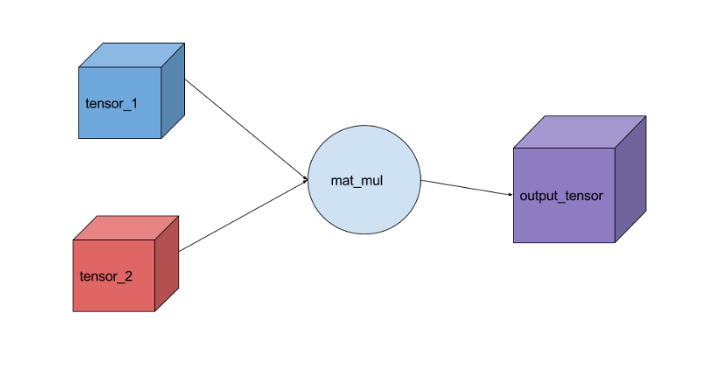
\includegraphics[width=6.5in]{images/tensor.png}
    \caption{Trivial tensor example.}
\end{figure}

The code above is creating two constant tensors and multiplying them together and outputting our result. This is a trivial example that demonstrates how you can create a graph and run the session. All inputs needed by the op are run automatically. They’re typically ran in parallel. This session run actually causes the execution of three operations in the graph, creating the two constants then the matrix multiplication.

\subsubsection{Graph}

The constants and operation was automagically added to the graph in TensorFlow. The graph default is instantiated when the library is imported. Creating a Graph object instead of using the default graph is useful when creating multiple models in one file that do not depend on each other.

\begin{lstlisting}[language=Python]
    new_graph = tf.Graph()
    with new_graph.as_default():
        new_g_const = tf.constant([1., 2., 3.])
\end{lstlisting}

any variables or operations used outside of the "with new\_graph.as\_default()" will be added to the default graph that is created when the library is loaded. You can even get a handle to the default graph with

\begin{lstlisting}[language=Python]
    default_g = tf.get_default_graph()
\end{lstlisting}

for most cases it’s best to stick with the default graph.

\subsubsection{Session}

This encapsulates the environment that operations and tensors are executed and evaluated. Sessions can have their own variables, queues and readers that are allocated. So it’s important to use the close() method when the session is over. There are 3 arguments for a Session, all of which are optional.

\begin{itemize}
    \item target: (Optional.) The execution engine to connect to. Defaults to using an in-process engine. 
    \item graph: (Optional.) The Graph to be launched. If no graph argument is specified when constructing the session, the default graph will be launched in the session. If you are using more than one graph (created with tf.Graph() in the same process, you will have to use different sessions for each graph, but each graph can be used in multiple sessions. In this case, it is often clearer to pass the graph to be launched explicitly to the session constructor.
    \item config: (Optional.) A ConfigProto protocol buffer with configuration options for the session.
\end{itemize}

\subsubsection{Placeholder}

As mentioned before, it all starts with placeholders. We need two placeholders in order to fit our model: X contains the network's inputs (the stock prices of all S\&P 500 constituents at time T = t) and Y the network's outputs (the index value of the S\&P 500 at time T = t + 1).

The shape of the placeholders correspond to [None, n\_stocks] with [None] meaning that the inputs are a 2-dimensional matrix and the outputs are a 1-dimensional vector. It is crucial to understand which input and output dimensions the neural net needs in order to design it properly.

\begin{lstlisting}[language=Python]
    # Placeholder
    X = tf.placeholder(dtype=tf.float32, shape=[None, n_stocks])
    Y = tf.placeholder(dtype=tf.float32, shape=[None])
\end{lstlisting}

The None argument indicates that at this point we do not yet know the number of observations that flow through the neural net graph in each batch, so we keep if flexible. We will later define the variable batch\_size that controls the number of observations per training batch.

\subsubsection{Variable}

Besides placeholders, variables are another cornerstone of the TensorFlow universe. While placeholders are used to store input and target data in the graph, variables are used as flexible containers within the graph that are allowed to change during graph execution. Weights and biases are represented as variables in order to adapt during training. Variables need to be initialized, prior to model training. We will get into that a litte later in more detail.

The model consists of four hidden layers. The first layer contains 1024 neurons, slightly more than double the size of the inputs. Subsequent hidden layers are always half the size of the previous layer, which means 512, 256 and finally 128 neurons. A reduction of the number of neurons for each subsequent layer compresses the information the network identifies in the previous layers. Of course, other network architectures and neuron configurations are possible but are out of scope for this introduction level article.

\begin{lstlisting}[language=Python]
    # Model architecture parameters
    n_stocks = 500
    n_neurons_1 = 1024
    n_neurons_2 = 512
    n_neurons_3 = 256
    n_neurons_4 = 128
    n_target = 1
    # Layer 1: Variables for hidden weights and biases
    W_hidden_1 = tf.Variable(
            weight_initializer(
                [n_stocks, n_neurons_1]))
    bias_hidden_1 = tf.Variable(
            bias_initializer(
                [n_neurons_1]))
    # Layer 2: Variables for hidden weights and biases
    W_hidden_2 = tf.Variable(
            weight_initializer(
                [n_neurons_1, n_neurons_2]))
    bias_hidden_2 = tf.Variable(
            bias_initializer(
                [n_neurons_2]))
    # Layer 3: Variables for hidden weights and biases
    W_hidden_3 = tf.Variable(
            weight_initializer(
                [n_neurons_2, n_neurons_3]))
    bias_hidden_3 = tf.Variable(
            bias_initializer(
                [n_neurons_3]))
    # Layer 4: Variables for hidden weights and biases
    W_hidden_4 = tf.Variable(
            weight_initializer(
                [n_neurons_3, n_neurons_4]))
    bias_hidden_4 = tf.Variable(
            bias_initializer(
                [n_neurons_4]))
    
    # Output layer: Variables for output weights and biases
    W_out = tf.Variable(
            weight_initializer(
                [n_neurons_4, n_target]))
    bias_out = tf.Variable(
            bias_initializer(
                [n_target]))
\end{lstlisting}

It is important to understand the required variable dimensions between input, hidden and output layers. As a rule of thumb in multilayer perceptrons (MLPs, the type of networks used here), the second dimension of the previous layer is the first dimension in the current layer for weight matrices. This might sound complicated but is essentially just each layer passing its output as input to the next layer. The biases dimension equals the second dimension of the current layer’s weight matrix, which corresponds the number of neurons in this layer.

\subsubsection{Scope}

Variables and tensors in TensorFlow have a name attribute that is used to identify them in the symbolic graph. If you don't specify a name when creating a variable or a tensor, TensorFlow automatically assigns a name for you:

\begin{lstlisting}[language=Python]
    a = tf.constant(1)
    print(a.name)  # prints "Const:0"
    
    b = tf.Variable(1)
    print(b.name)  # prints "Variable:0"
\end{lstlisting}

You can overwrite the default name by explicitly specifying it:

\begin{lstlisting}[language=Python]
    a = tf.constant(1, name="a")
    print(a.name)  # prints "a:0"
    
    b = tf.Variable(1, name="b")
    print(b.name)  # prints "b:0"
\end{lstlisting}

TensorFlow introduces two different context managers to alter the name of tensors and variables. The first is tf.name\_scope:

\begin{lstlisting}[language=Python]
    with tf.name_scope("scope"):
    a = tf.constant(1, name="a")
    print(a.name)  # prints "scope/a:0"
    
    b = tf.Variable(1, name="b")
    print(b.name)  # prints "scope/b:0"
    
    c = tf.get_variable(name="c", shape=[])
    print(c.name)  # prints "c:0"
\end{lstlisting}

Note that there are two ways to define new variables in TensorFlow, by creating a tf.Variable object or by calling tf.get\_variable. Calling tf.get\_variable with a new name results in creating a new variable, but if a variable with the same name exists it will raise a ValueError exception, telling us that re-declaring a variable is not allowed.

tf.name\_scope affects the name of tensors and variables created with tf.Variable, but doesn't impact the variables created with tf.get\_variable.

Unlike tf.name\_scope, tf.variable\_scope modifies the name of variables created with tf.get\_variable as well:

\begin{lstlisting}[language=Python]
    with tf.variable_scope("scope"):
        a = tf.constant(1, name="a")
        print(a.name)  # prints "scope/a:0"
        
        b = tf.Variable(1, name="b")
        print(b.name)  # prints "scope/b:0"
        
        c = tf.get_variable(name="c", shape=[])
        print(c.name)  # prints "scope/c:0"
  
    with tf.variable_scope("scope"):
        a1 = tf.get_variable(name="a", shape=[])
        a2 = tf.get_variable(name="a", shape=[])  # Disallowed
\end{lstlisting}

But what if we actually want to reuse a previously declared variable? Variable scopes also provide the functionality to do that:

\begin{lstlisting}[language=Python]
    with tf.variable_scope("scope"):
        a1 = tf.get_variable(name="a", shape=[])
    with tf.variable_scope("scope", reuse=True):
        a2 = tf.get_variable(name="a", shape=[])  # OK
\end{lstlisting}

\subsubsection{Loss}

Loss is the target function that the optimization algorithm will try to minimize.

In general, you want your loss function to be a measure of how bad your model is. But because the optimization algorithms require a few mathematical properties to work nicely, you can't pick the usual stuff like precision and recall (you want continuous functions that are differentiable in relation to the model parameters).

With classification tasks, softmax is a common choice. It's a smooth and well-behaved version of argmax, which is used to pick the class with highest network activation. With regression, the usual mean squared error serves fine.

\subsubsection{Logits}

Logit is a function. This will map probabilities [0, 1] to [-inf, +inf].

Softmax is a function that maps [-inf, +inf] to [0, 1] similar as Sigmoid. But Softmax also normalizes the sum of the values(output vector) to be 1.

Tensorflow "with logit": It means that you are applying a softmax function to logit numbers to normalize it. The input\_vector/logit is not normalized and can scale from [-inf, inf].

For multiclass classification problems is used this normalization. And sigmoid normalization is used for multilabel classification problems i.e. 
\begin{lstlisting}[language=Python]
    tf.nn.sigmoid_cross_entropy_with_logits
\end{lstlisting}

\subsubsection{Feed}

There are three main methods of getting data into a TensorFlow program:

\begin{itemize}
    \item Feeding: Python code provides the data when running each step.
    \item Reading from files: an input pipeline reads the data from files at the beginning of a TensorFlow graph.
    \item Preloaded data: is a constant or a variable in the TensorFlow graph that holds all the data (for small data sets).
\end{itemize}

TensorFlow's feed mechanism lets you inject data into any Tensor in a computation graph. A python computation can thus feed data directly into the graph.

Supply feed data through the feed\_dict argument to a run() or eval() call that initiates computation.

\begin{lstlisting}[language=Python]
    with tf.Session():
        input = tf.placeholder(tf.float32)
        classifier = ...
        print(classifier.eval(
            feed_dict={input: 
                my_python_preprocessing_fn()}))
\end{lstlisting}

\subsubsection{Tensor}

All you need to describe a tensor fully is its data type and the value of each of the N dimension. Very briefly, a tensor is an N-dimensional array containing the same type of data (int32, bool, etc.).

That’s why we describe a tensor with what we call a shape: it is a list, tuple or TensorShape of numbers containing the size of each dimension of our tensor, for example:

\begin{itemize}
    \item For a tensor of n dimensions: (D0, D1, …, Dn-1)
    \item For a tensor of size W x H (usually called a matrix): (W, H)
    \item For a tensor of size W (usually called a vector): (W,)
    \item For a simple scalar (those are equivalent): () or (1,)
\end{itemize}

Note: (D*, W and H are integers)

Note on the vector (1-D tensor): it is impossible to determine if a vector is a row or column vector by looking at the vector shape in TensorFlow, and in fact it doesn’t matter. 

A tensor looks like this in TensorFlow:

\begin{lstlisting}[language=Python]
    import tensorflow as tf

    my_tensor = tf.constant(0., shape=[6,5,8])
    print(my_tensor) 
    # -> Tensor("Const:0", shape=(6, 5, 8), dtype=float32)
\end{lstlisting}

\subsubsection{Static shape}

The static shape is the shape you provided when creating a tensor OR the shape inferred by TensorFlow when you define an operation resulting in a new tensor. It is a tuple or a list.

TensorFlow will do its best to guess the shape of your different tensors (between your different operations) but it won’t always be able to do it. Especially if you start to do operations with placeholder defined with unknown dimensions (like when you want to use a dynamic batch size).

To use the static shape (Accessing/changing) in your code, you will use the different functions which are attached to the Tensor itself and have an underscore in their names:

\begin{lstlisting}[language=Python]
    import tensorflow as tf

    # I create a first Tensor with a defined shape
    my_tensor = tf.constant(0, shape=[6,2])
    my_static_shape = my_tensor.get_shape()
    print(type(my_static_shape)) 
    # -> TensorShape
    # Full description: TensorShape([Dimension(6), Dimension(2)])
    
    print(my_static_shape) 
    # -> (6, 2)
    
    # You can get it as a list too
    print(my_static_shape.as_list()) 
    # -> [6, 2]
    
    # Let's do an operation resulting in a new tensor
    my_tensor_transposed = tf.transpose(my_tensor)
    print(my_tensor_transposed.get_shape()) 
    # -> (2, 6)
    # The static shape has been inferred by 
    #   TensorFlow based on the transpose operation 
    # and the tensors used by the operation
    
    # At any moment, you can also force 
    # a Tensor with an undefined (None) dimension
    # to have a precise shape of the same rank.
    my_placeholder = tf.placeholder(tf.float32, shape=[None, 2])
    print(my_placeholder.get_shape()) 
    # -> [?, 2]
    
    my_placeholder.set_shape([8, 2])
    print(my_placeholder.get_shape()) 
    # -> [8, 2]
\end{lstlisting}

Note: The static shape is very useful to debug your code with print so you can check your tensors have the right shapes.

\subsubsection{Dynamic shape}

The dynamic shape is the actual one used when you run your graph. It is itself a tensor describing the shape of the original tensor.

If you defined a placeholder with undefined dimensions (with the None type as a dimension), those None dimensions will only have a real value when you feed an input to your placeholder and so forth, any variable depending on this placeholder.

To use the dynamic shape(Accessing/changing) in your code, you will use the different functions which are attached to the main scope and don’t have an underscore in their names:

\begin{lstlisting}[language=Python]
    import tensorflow as tf

    # Tensor('Const:0' shape=(6, 2) dtype=int32)
    my_tensor = tf.constant(0, shape=[6 ,2]) 
    my_dynamic_shape = tf.shape(my_tensor) 
    print(my_dynamic_shape)
    # -> Tensor('Shape:0' shape=(2,) dtype=int32)
    # The shape of the tensor "Shape" is (2,) 
    # because my_tensor is a 2-D tensor
    # so the dynamic shape is a 1-D tensor
    # containing sizes of my_tensor dimensions
    # and in this case, we have 2 dimensions.
    
    my_reshaped_tensor = tf.reshape(my_tensor, [2, 3, 2]) 
    print(my_reshaped_tensor)
    # -> Tensor('Reshape:0' shape=(2, 3, 2) dtype=int32)
    
    # To access a dynamic shape value, you need to run 
    # your graph and feed any placeholder 
    # that your tensor my depended upon:
    print(my_dynamic_shape.eval(session=tf.Session(), feed_dict={
        my_tensor: [[1., 2.], [1., 2.], [1., 2.], 
        [1., 2.], [1., 2.], [1., 2.]]
    }))
    # -> [6, 2]
\end{lstlisting}

The dynamic shape is very handy for dealing with dimensions that you want to keep dynamic.
